\section{Resultados}
\subsection{Polinômios geradores e distâncias mínimas}
Os polinômios geradores utilizados e suas respectivas distâncias mínimas de código associado são mostradas em Listagem \ref{lst:polinomios}. Os índices são os mesmos do conjunto $S$ apresentado junto ao algoritmo. As distâncias mínimas, com mesma indexação de $S$ foram $\{2, 4, 3, 4, 2\}$.

\begin{align}
	\nonumber
	p_1 = D^4+D^3+D^2+D+1\\ \nonumber
	p_2 = D^5+D^3+D^2+1\\ \nonumber
	p_3 = D^6+D^2+1\\ \nonumber
	p_4 = D^6+D^4+D^3+D^2+1\\
	p_5 = D^7+D^6+D^5+D^4+D^3+D^2+D+1
	\label{lst:polinomios}
\end{align}

\subsection{\label{complexidade_decod}Complexidade de decodificação BCH}

Segundo \cite{ref:algoritmo-berlekamp}, a decodificação de códigos BCH se dá em $O(n)$, $n$ sendo o tamanho de bloco empregado. Para confirmar a validade dessa afirmação, construíram-se códigos $BCH(m, 3)$, com $m \in \lbrace 4,5,...,20 \rbrace$, e mediram-se os tempos de decodificação submetendo a mesma palavra a cada um deles, com resultados ilustrados pela Figura \ref{fig:bch_decoding_is_linear}.

\begin{figure}[!hb]
	\centering
    \captionsetup{justification=centering}
	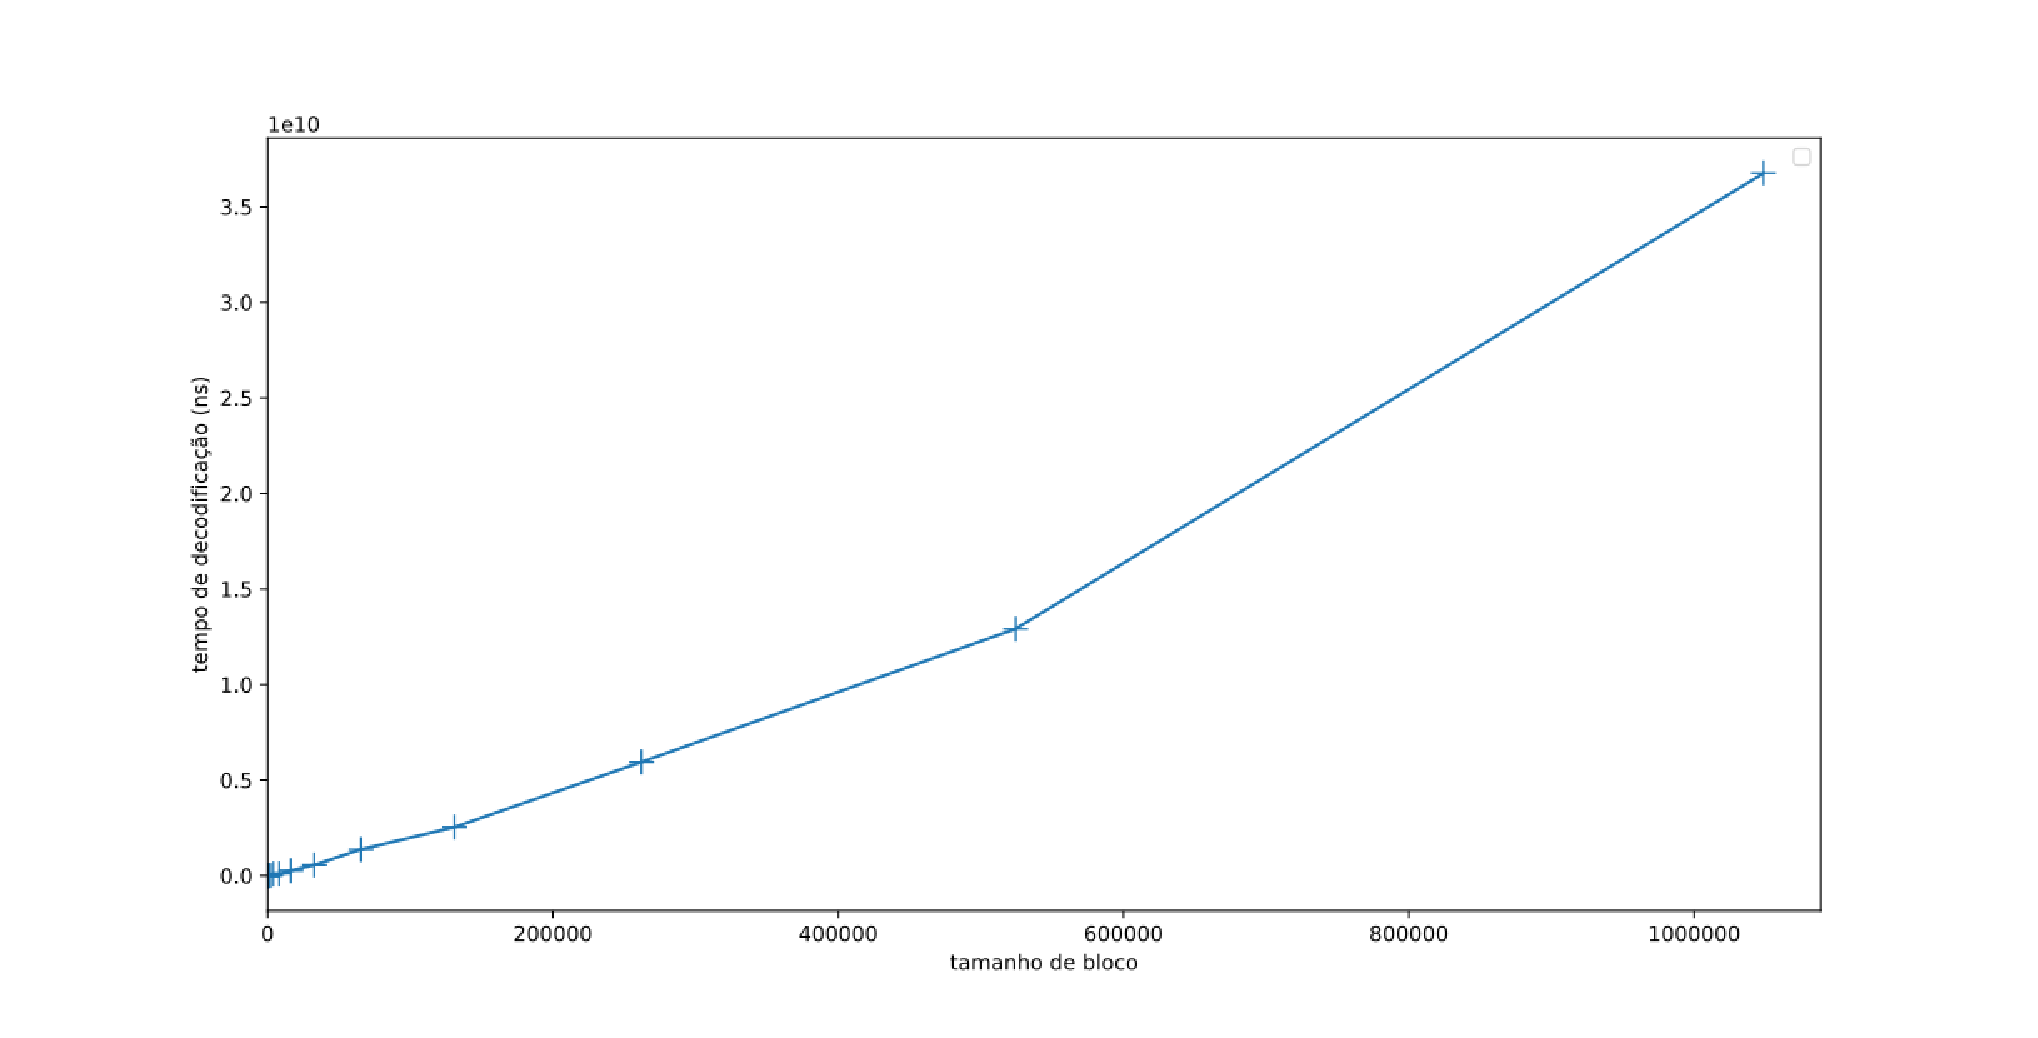
\includegraphics[scale=0.3]{floats/bch-decode-is-linear.eps}
	\caption{\label{fig:bch_decoding_is_linear}Tempo de decodificação para BCH com variados tamanhos de bloco.}
\end{figure}